\documentclass{article}
\usepackage[utf8]{inputenc}
\usepackage{amsmath}
\usepackage{dirtytalk}
\usepackage{graphicx}
\usepackage{hyperref}
\usepackage{mathtools}
\usepackage{natbib}
\usepackage{float}
\usepackage{subcaption}
\usepackage{caption}
\usepackage{wrapfig}
\usepackage{listings}
\graphicspath{ {./images/} }
\DeclareMathSizes{15}{30}{16}{12}
\DeclareMathOperator{\spn}{span}
\usepackage[a4paper, total={6.5in, 8in}]{geometry}

\title{\Huge Hw 1 Exercise 1}
\author{\huge Dylan Lyon}

\let\oldquote\quote
\let\endoldquote\endquote
\renewenvironment{quote}[2][]
  {\if\relax\detokenize{#1}\relax
     \def\quoteauthor{#2}%
   \else
     \def\quoteauthor{#2~---~#1}%
   \fi
   \oldquote}
  {\par\nobreak\smallskip\hfill(\quoteauthor)%
   \endoldquote\addvspace{\bigskipamount}}

\begin{document}

\maketitle

\section{Overview}\\

Hello! My research is in higher-order geometry generation for differential modelers, primarily with solid mechanics and HXfer applications. The method used is localized collocation meshless method, a nifty irregular approach to finite difference modelling that gets derivatives using a static set of neighbor nodes for every node (i.e. not different neighbors in x,y,z - Same p neighbors with different weightings for each derivative). Lends itself to higher orders because of meshless property, i.e. no factorial scaling with more dimensions.\\

Application is generative design. Softwares like AutoCAD and AxSTREAM create discrete geometries, simulate to test some objective function, and interpolate this function. Each distinct geometry has design parameters $\overline{\alpha} = \left[ \alpha_0 , \alpha_1 , .. \alpha_m \right]^T$. The stated goal is to find some $\overline{\alpha} \in \spn \left[\alpha \right] \ni f(\overline{\alpha}) = \inf f$.\\

But there's a silly bottlenecking there: Interpolating over discrete $\overline{\alpha}$ to then run another simulation of a different geometric space $\overline{x} \in \mathbb{R}^n$. Using a more general differential equation in both $\overline{x}$ and $\overline{\alpha}$ lends itself to a PDE solution that is differentiable over $\alpha$ space, where $f$ extrema can be found quickly. In time notation that's:\\
\begin{align*}
\mathcal{O}\left(\text{FEM}(\overline{x}) \bigotimes \text{Latin Space} (\overline{\alpha})\right) & & \text{vs} & & \mathcal{O}\left(\text{LCMM}(\overline{x},\overline{\alpha})\right)
\end{align*}
An excellent book that I learned LCMM from is Pepper et al.\cite{pepper_kassab_divo_2014}. Great, great book that develops a modern LCMM implementation with codes in an engineering environment. LCMM is proposed here and in the book as a way to sidestep factorial coefficients in higher spaces, exampled below.\\
\begin{figure}[H]
\begin{center}
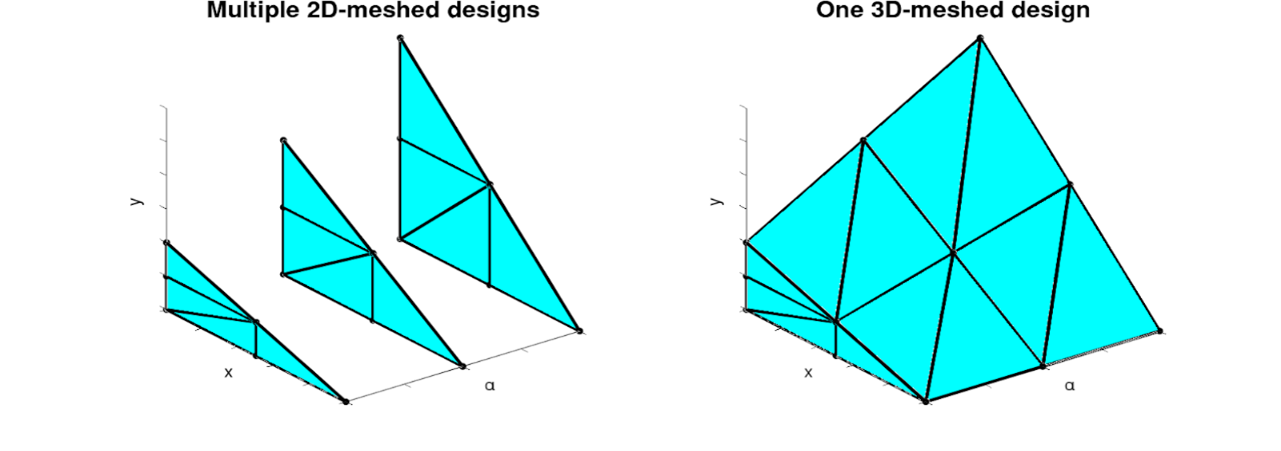
\includegraphics[width=5in,center]{triangle meshes.png}
    \caption{Multiple 2D meshes vs combined 3D mesh. Notice 4 faces instead of 1 per simplex.}
\label{fig:foo}
\end{center}
\end{figure}
\section{Implementation}
An example here is that of heat transfer over a 2D right triangular fin with variable height in y-axis (See ~\ref{fig:foo}). This variable height serves as a single $\alpha$ design parameter, for a total of 3 dimensions. The bottom edge is heated, left edge is adiabatic, and hypotenuse edge is cooled by $+x$ forced and natural convection. There exists an optimum $\alpha$ that maximizes the convective hxfer coefficient $h$ on this edge. A traditional discrete optimization would be generating 2D meshes of various $\alpha$, running a heat transfer code, and interpolating over the convection coefficients for each geometry. Adapt/refine if necessary. My approach will create a 3D meshless model, solve over nodes in the $\left( \overline{x},\overline{\alpha}\right)$ space, and then retrieve an $\alpha$ solution. Adapt/refine if necessary.\\
\subsection{PDE}
Use simple steady-state heat transfer equation:\\
\begin{equation}
    \rho c_P \frac{\partial T}{\partial t} = 0 (WK/m^3) = \sum_{\hat{j}\in \hat{X}} k \frac{\partial ^2 T}{\partial x_{\hat{j}}^2}
\end{equation}

Cool, now a major fault in my plan is exposed: Transient solutions, which would require iterations (explicit) or node creation (implicit) over a larger space than $\overline{x}$ and efficiency is damaged. Not good!\\

Another, less obvious fault is that established work and codes in boundary condition treatment requires additional effort to define. BC's need to be defined over the hypotenuse in the $\left( \overline{x},\overline{\alpha}\right)$ space, not just in $\left( \overline{x}\right)$.\\

\subsection{LCMM}
Below~\ref{lst:code} is an object-level skeleton of LCMM. Similar to skeleton given in \cite{lcmm}.
\begin{lstlisting}[label={lst:code},caption={Node struct in LCMM}]
struct Node : A node in LCMM with PDE function value (Temperature)
    int p : Number of nodes in p family
    int* pfamily : Pointer array to nodes in p family
    float64* coeffs : PDE coefficients at this node (Here, k)
    float64 c : LCMM weighting inverse multiquadric coefficient
    float64* ws : Weightings of p family nodes
    
    @func void buildEqn : Add equation to linear system
    @func float64* weightings : Populates ws variable
end
\end{lstlisting}


\bibliographystyle{IEEEtran} % We choose the "plain" reference style
\bibliography{dslyon_Ex1} % Entries are in the refs.bib file

\end{document}
